\section{Methods}
We develop a recurrent variational autoencoder to model gene expression dynamics (RVAgene). Here we briefly describe the methods underpinning variational autoencoders, and present the implementation of RVAgene. 

\subsection{Variational inference and variational autoencoders}
In the most general setting of a Bayesian model, we seek to learn the latent variables $\vz$ that best characterize some data $\vx$. Given a generative process that draws latent variables from a prior distribution, $p(\vz)$, and a likelihood of the data observed that is given by $p(\vx|\vz)$, then the posterior probability is given by Bayes rule:
%Our target is to learn about $\vz$ given the observed $\vx$, which is governed simply by the Bayes' rule:
\begin{align*}
 p( \vz | \vx)&= \frac{p(\vx|\vz)p(\vz)}{\int_z p(\vx|\vz)p(\vz) dz}. \numberthis \label{bayes-rule}
\end{align*}
The denominator is often intractable, making it difficult to estimate $p( \vz | \vx)$. Markov Chain Monte Carlo methods provide means to estimate posterior probability distributions. 
An alternative method to estimate hard-to-compute probability distributions is Variational Inference (VI) \citep{Hoffman2013}, which starts from the assumption that the posterior can be approximated by a distribution $q(\vz)$ from the family $\cQ$. VI then amounts to an optimization problem to find the $q^*$ that minimizes the Kullback–Leibler (KL) divergence between the approximation and the true posterior: 
\begin{align*}
 q^*(\vz) &= \textrm{argmin}_{q(\vz)\in\cQ} \textrm{KL}(q(\vz)||p(\vz|\vx)). \numberthis \label{vi-formulation}
\end{align*}

Much recent effort has gone into solving VI problems in different settings \citep{Zhang2019,
Ingraham2017, Bouchard-Cote2010}. VI can be framed as solving an optimization problem over function
families: neural networks are popular candidates for representing and learning complex functions. VI
was incorporated into autoencoders \citep{Kingma2014} to create the architecture of a variational
autoencoder (VAE). A VAE consists of an encoder network to approximate $p(\vz|\vx)$ through a
function $q_\vx(\vz)$, and a decoder network $p(\vx|\vz)$ (fig. \ref{fig:fig2}). Conceptually, the encoder solves an inference problem: approximating the posterior distribution $p(\vz|\vx)$ as some $q^*_\vx(\vz)$, while the decoder solves a reconstruction problem: defining a generative process for $p(\vx|\vz)$, given the latent variables.
The VAE posterior is modeled by a multivariate normal $\cN(\mathbf{\mu},\Sigma)$ of the same dimension as $\vz$. Training then comes down to minimizing two objective functions. For the encoder network, which should learn a ``well distributed'' latent space, minimize the KL divergence: KL$(\cN(\mathbf{\mu},\Sigma) || \cN(0,\vI)) $. For the decoder network, which should reconstruct the inputs $\vx$ from the latent space, minimizing either an $L1$ or $L2$ objective function with respect to $\hat{\vx}$ is appropriate. The use of KL-divergence and an $L2$ objective solves the VI formulation of Eq. \ref{vi-formulation} \citep{Kingma2014}, however, an $L1$ objective may be preferred in practice, e.g. in cases where we want to suppress the effects of outliers on the structure of $\vz$ \citep{botchkarev2018performance}.

% Each input point $\vx_i$ is encoded as a distribution over the latent space $\vz$ given a prior, \tcr{and also project $\vx_i$ to a point $\vz_i$ using the reparametrization trick (\cite{Kingma2014}).} Typically, VAEs typically use a standard normal prior $\cN(0,\vI)$ as the prior distribution over the latent space. The decoder network then takes points from the latent space $\vz$ as input, and generates $\vx$. 


%\begin{center}
%% 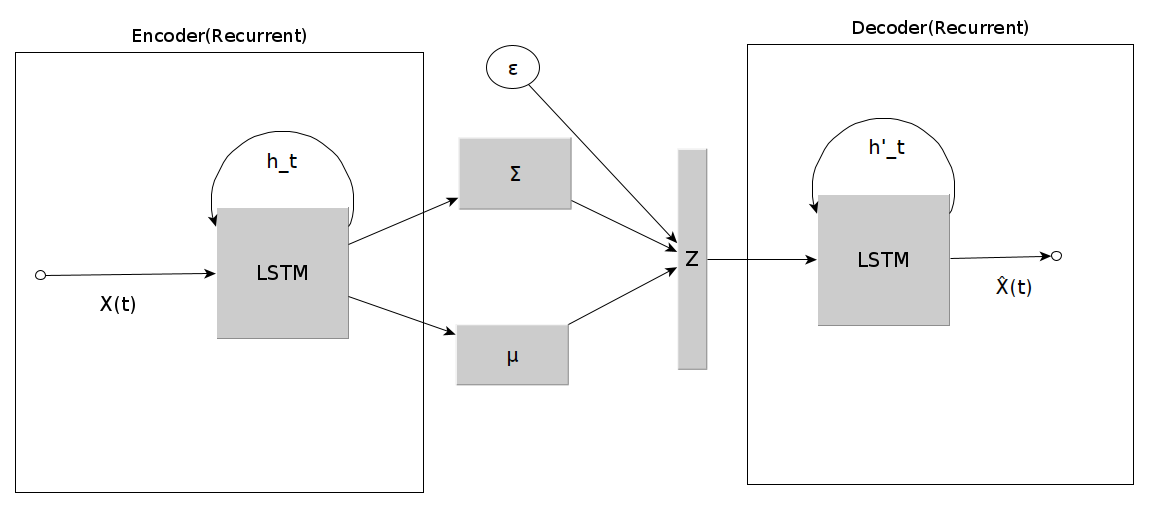
\includegraphics[scale=0.3]{architecture.png} 
%\begin{figure}
%\centering
%  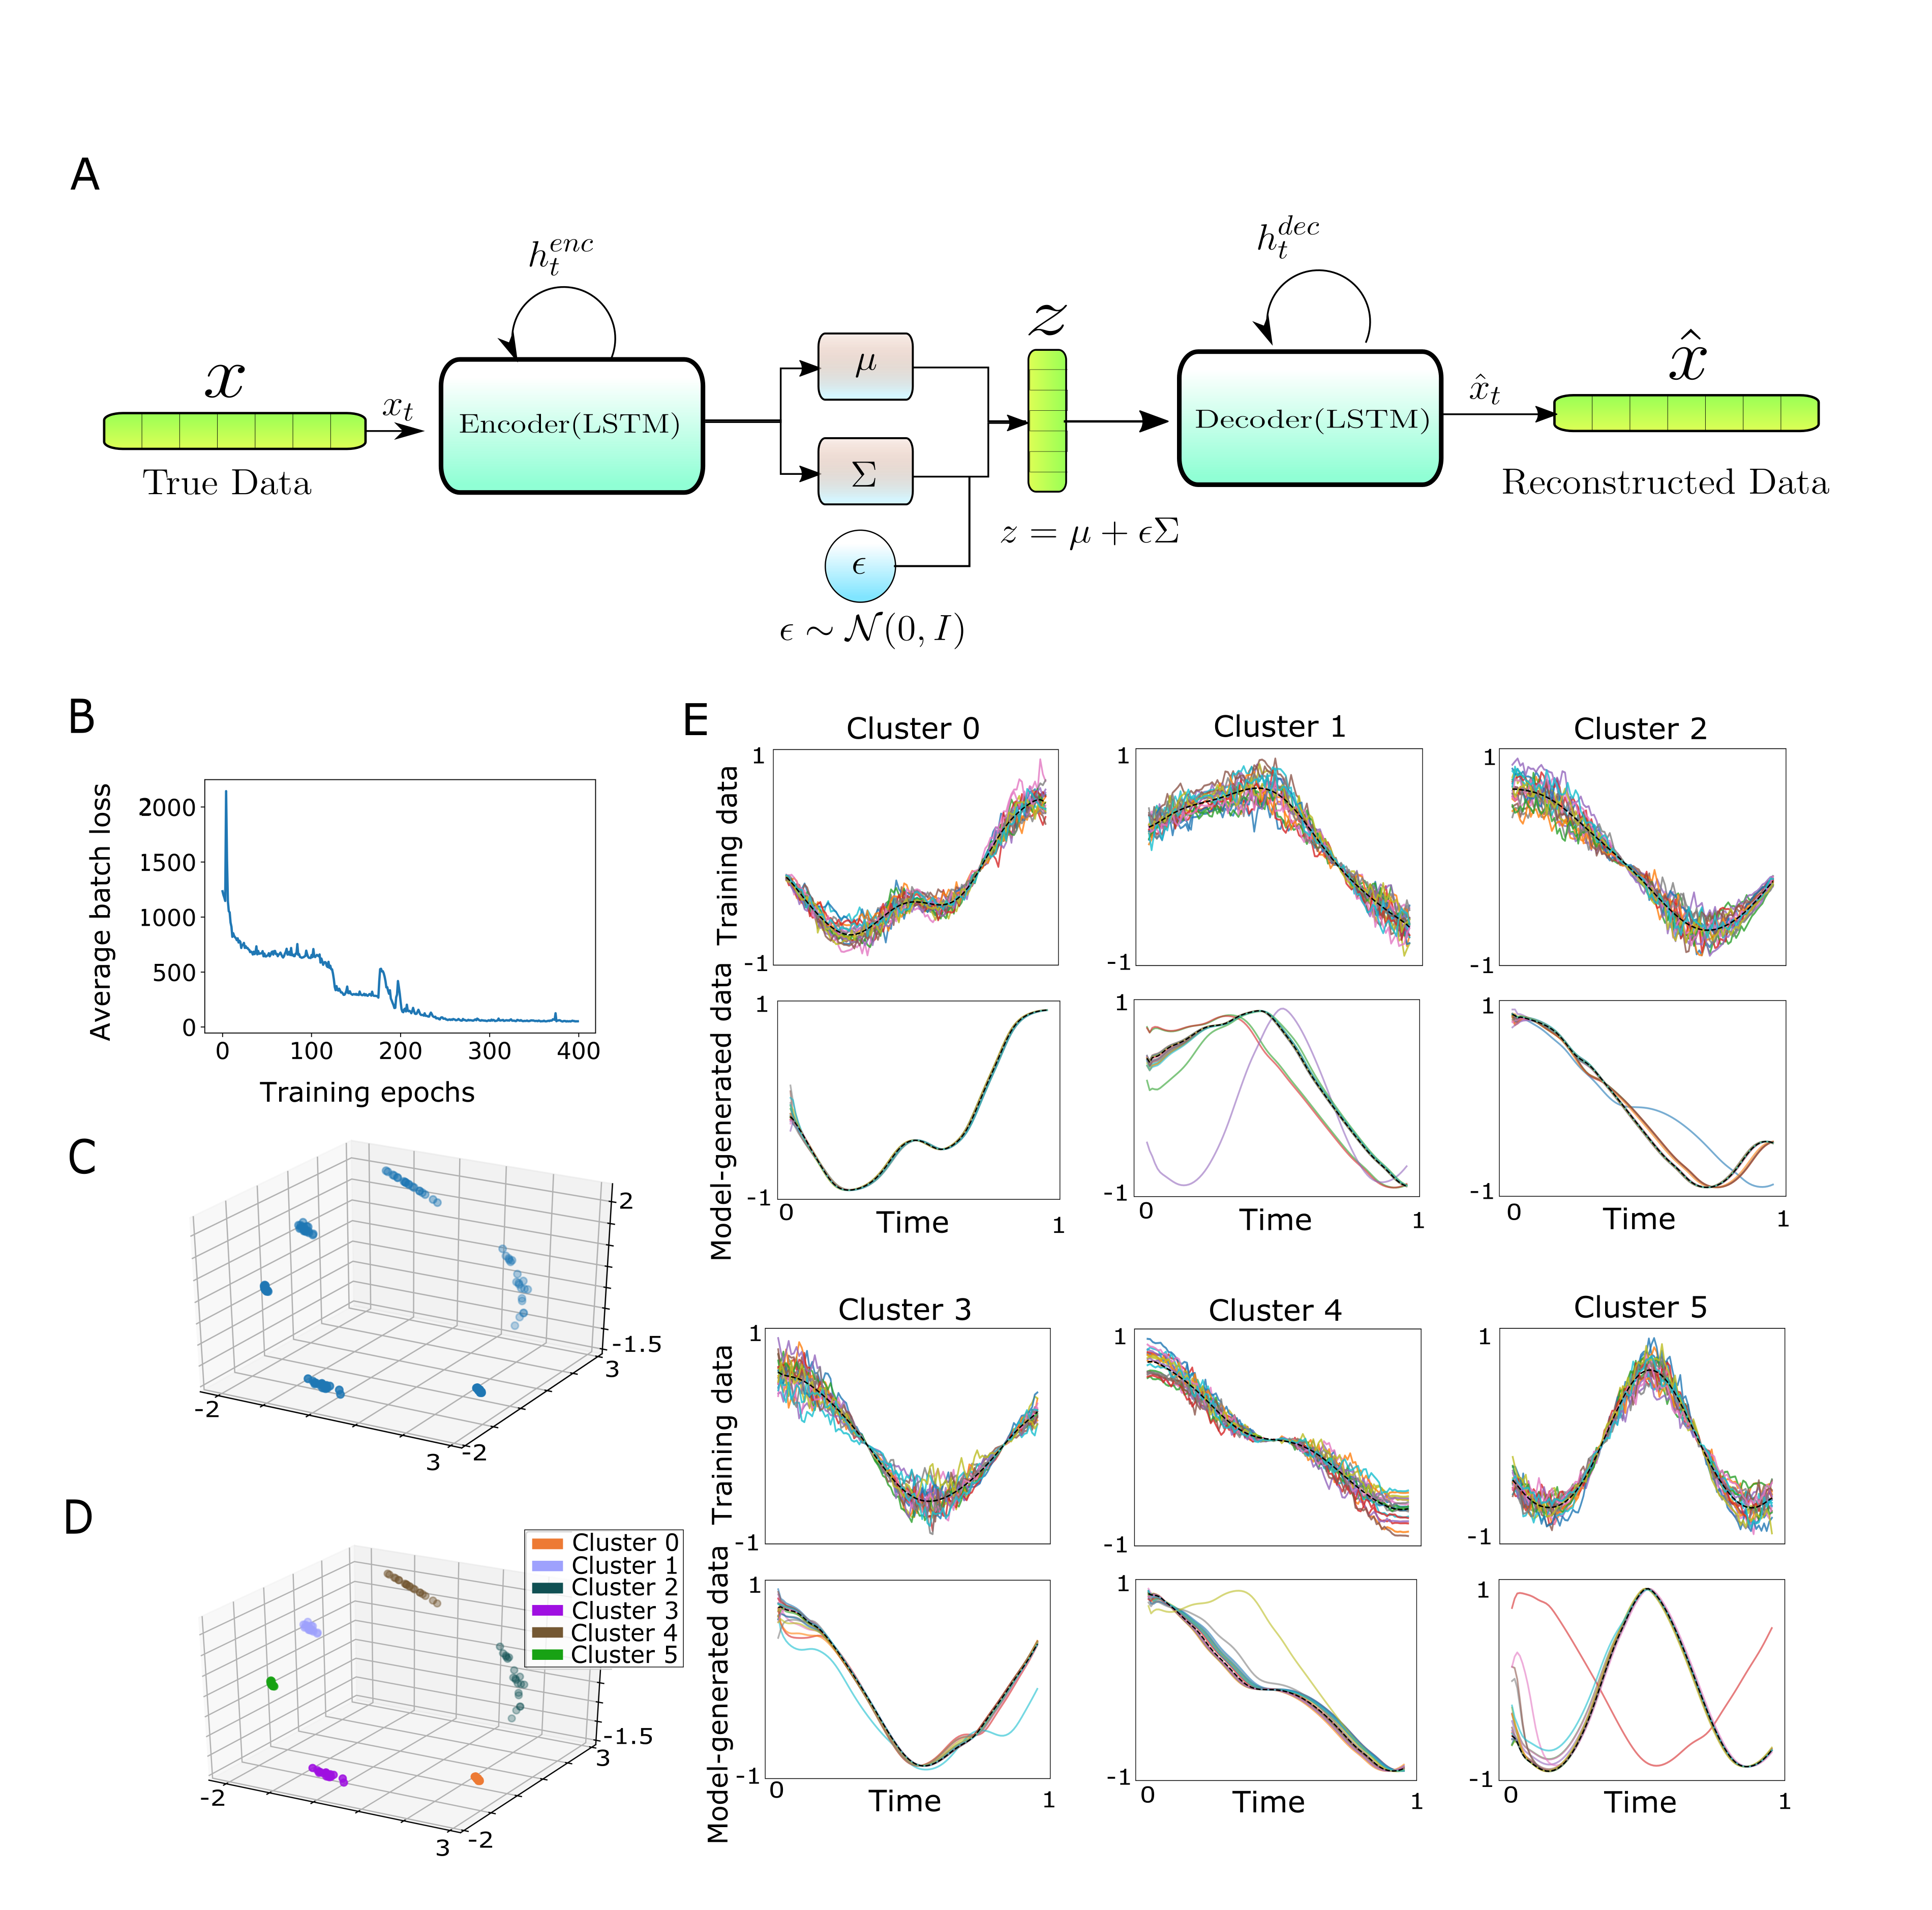
\includegraphics[width=\linewidth]{figures/fig1.png}
% % archetecture.png: 1149x508 px, 72dpi, 40.53x17.92 cm, bb=0 0 1149 508
% \caption{Schematic diagram of RVAgene.}
% \label{fig:scheme}
%\end{figure}
%\end{center}


%% Probably too much detail here, but may want to cite the refs. 
%So far, we haven't specified anything about architecture of the encoder and decoder networks of a VAE, except that they learn certain functions modelling the posterior and likelihood probabilities  of our generative story of the data we are interested in. In general we could make them a fully connected neural network. But, since we are interested in handling sequential (time-series) data, we expect a specific structure of those functions. Intuitively, the $t$-th time point of input sequenece $\vx$ should be causally dependent only on its previous timepoints (upto $t-1$).  Therefore, instead of designing a completely agnostic network (e.g. fully connected layers), we can use a recurrent architecture for the encoder and decoder, which are well established in modelling sequence data (e.g. text data (\cite{Nallapati2016}), time-series data (\cite{Malhotra2015})). This in essence reduces the search space of the model from completely agnostic to a family of recurrent functions.
%\cite{Fabius2015} used this idea and showed how Recurrent Variational Autoencoders can be useful as a unsupervised latent representation learning and generative model for music data.


\subsection{RVAgene: A recurrent variational autoencoder to model gene expression dynamics}
Following the VAE architecture, RVAgene consists of an encoder and a decoder network with a reparameterization step in between. To incorporate the knowledge that we are modeling temporal data, recurrent neural networks offer an ideal architecture to use for both the encoder and the decoder networks. Recurrent and VAE networks have been successfully combined elsewhere, e.g. for textual \citep{Nallapati2016} and time series data \citep{Malhotra2015}.
\par
The architecture of RVAgene is based on \citet{Fabius2015}. An input sequence (i.e. gene) $x \in \vx$, $x = (x_1,x_2,...,x_t,...,x_T)$ is encoded using a recurrent function described by a long short-term memory (LSTM) unit. LSTM units are the state-of-the-art in recurrent architectures, since they are robust against the vanishing gradient problem for longer sequences, unlike other recurrent units (see details in \citet{Hochreiter1997}). We encode $x$ in the following manner:
\begin{align*}
 h_{t+1}^{enc} &= \textrm{LSTM}(W_{enc}^Th_t^{enc} + W_{inp}^T{x_t}+b_{enc}), \numberthis \label{lstm}
\end{align*}
where ($W_{enc}$, $W_{inp}$ and $b_{enc}$) are network weight parameters, and the hidden states $h_t$ represent information shared over timepoints in the LSTM. The dimension of the $h_t$ (and  $W_{enc}$) is given by a hyperparameter (``hidden-size''). The encoded $h_{t+1}$ are used to parametrize the posterior mean and variance from $x$, with mean $\mu_z$ and diagonal covariance $\sigma_z$ as:
%represent this mean and diagonal covariance matrix of the normal distribution an input $x$ is getting encoded to. 

\begin{align*}
 \mu_z &= W_{\mu}^Th_{T+1}^{enc} + b_{\mu} \numberthis \label{mu}\\
  log(\sigma_z) &= W_{\sigma}^Th_{T+1}^{enc} + b_{\sigma}.  \label{sigma}
 \end{align*}
We then use the reparameterization step described in \citet{Kingma2014} to sample $z$ from the distribution:
\begin{align*}
 z = \mu_z + \epsilon\sigma_z, \numberthis 
\end{align*}
where, for known $\epsilon$, backpropagation through the sampling step is possible while training the network.
\par
For the decoder network, the first state $h_1$ is calculated from $z$, and the recurrent formulation follows by reconstructing $x$ as $\hat{x} = (\hat{x}_1,\hat{x}_2,...,\hat{x}_t,...,\hat{x}_T )$, thus:
\begin{align*}
 h_1^{dec} &= \textrm{sigm}(W_{z}^Tz + b_{z})   \\
h_{t+1}^{dec} &= \textrm{LSTM}(W_{dec}^Th_t^{dec} + W_{out}^T{\hat{x}_t}+b_{dec}) \numberthis \label{decoder_lstm} \\
\hat{x}_t &= \textrm{sigm}(W_{out}^Th_t^{dec} + b_{out}), \\
\end{align*}
where $\textrm{sigm}(u) = \frac{1}{1 + e^{-u}}$ is the sigmoid activation function, and ($W_i, b_i$)
are the network weight parameters. A schematic diagram of the network is shown in
\hyperref[fig:fig2]{Fig. 1.1A}, which can now be trained using backpropagation, to minimize the objective function: 
\begin{align*}
    \cL(\theta, x) = D_{KL}(\cN(\mathbf{\mu}_z,\Sigma_z)||\cN(\mathbf{0},\vI)) + |x - \hat{x}|, \numberthis \label{lossfunction}
\end{align*}
where $\mathbf{\mu}_z$ and $\Sigma_z = \textrm{diag}(\sigma_z)$ are calculated from $x$ by the encoder.
\par 
To evaluate the accuracy of RVAgene, we need an appropriate error measure. For each gene in the test set, we calculate the $L1$ reconstruction error between generated data $\hat{x}$ and true data $x$, averaged over all time points. We normalize the data to lie in $[0,1]$ to avoid skewing the error by differences in gene expression magnitudes. Thus we define:
\begin{align}
    \textrm{Reconstruction error}(x,\hat{x}) = \frac{1}{T}\sum_{t}| s(\hat{x})_t - s(x)_t |,  & \text{ where } s(x) = \frac{x}{\sum_{t=1}^Tx_t}.
\end{align} 

\subsection{Generating synthetic gene expression time series data}
To test RVAgene, we generate a synthetic time series dataset. Six clusters each containing 20 genes are simulated, where for each cluster $c$, the mean gene expression time series $Y_c = (y_{c1}, y_{c2}, ..., y_{ct})$ was generated using addition or convolution and rescaling of two random sinusoidal functions of the form $k_1\textrm{sin}(k_2t)$, where $k_1,k_2$ are randomly chosen positive integers. Trajectories of cluster members were then generated by sampling from the multivariate normal $\cN(Y_c,\Sigma_c)$. We model $\Sigma_c$ as the positive definite matrix $\alpha Y_cY_c^T$, where $\alpha$ is a scaling factor, we use: $\alpha = 1/|Y_c Y_c^T|$. As defined, $\Sigma_c$ will describe nonzero correlations for all pairs of time points, $(t_i,t_j)$. This is unrealistic, so we set to 0 the entries of $\Sigma_c$ for which column and row indices have a difference of more than some threshold $T$ (we used $T=50$), reflecting the fact that correlations between time points are lost over larger time windows (temporal correlations are local). Note that under this condition, $\Sigma_c$  is no longer necessarily positive definite. The multivariate Gaussian sampler \verb+numpy.random.multivariate_normal()+ implemented in \verb+numpy+ \citep{harris2020array} was used to sample from this augmented $\Sigma_c$.
{After generating a simulated dataset by this process, we also added Gaussian noise, drawn from $\cN(0,0.7)$, to the simulated dataset to produce an additional dataset exhibiting higher levels of noise.}

